\chapter{Additive Manufacturing}
Dit is een redelijk nieuwe technologie, gaat vooral over 3D-printen.
Ferrari 3D print een deel van hun motoren voor hun formule 1 wagens, dit is lichter en gaf hun de optie om legeringen te maken door laag per laag van composiet te veranderen. Ze kunnen ook complexe geometrieën maken die niet mogelijk zijn met traditionele productietechnieken. Dit is wel geen 'series production' (ze maken maar 1 motor per jaar), maar het is wel een voorbeeld van hoe additive manufacturing kan worden gebruikt in de industrie.
Het bedrijf relativity maakt raketten met 3D-printen, ze kunnen een raket in 60 dagen maken, terwijl dit normaal 2 jaar duurt. Ze kunnen ook complexe geometrieën maken die niet mogelijk zijn met traditionele productietechnieken. (VOLLEDIGE RAKETTEN)
Huizen kunnen ook ge 3D-print worden met beton.
Dit waren dus voorbeelden, 1 nadeel is de waste, dus de supports eigelijk, dit is verspilt materiaal, maar dit is wel nodig om de geometrie te kunnen maken. Er zijn ook technieken die dit probleem proberen op te lossen, zoals het gebruik van oplosbare supports of het gebruik van materialen die kunnen worden gerecycled. Het is ook een zeer digitaal manufacturing proces want je sliced je model eigelijk in software en dan print je laag per laag, dus er is veel controle over het proces en de geometrie die je kan maken. Er zijn ook veel verschillende materialen die kunnen worden gebruikt, zoals metalen, kunststoffen, keramiek, \dots
Er zijn verschillende benamingen hiervoor, ik ga ze niet allemaal bespreken maar hier is de slide:
\begin{figure}[H]
  \centering
  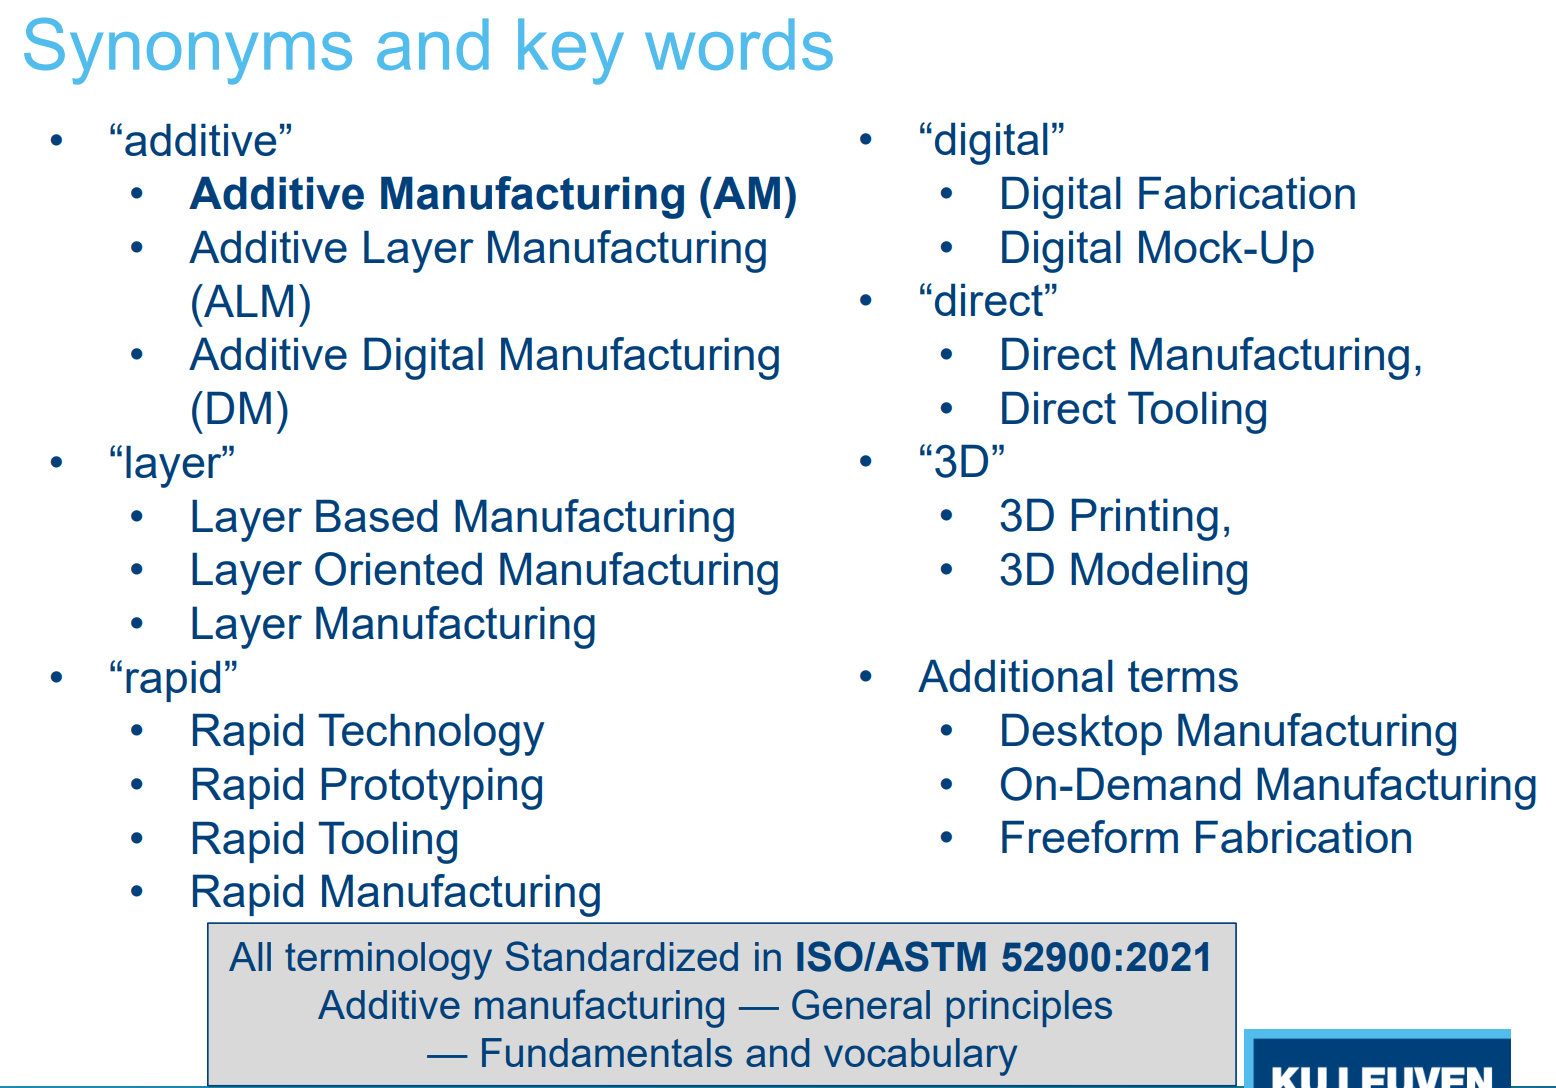
\includegraphics[width=0.5\textwidth]{assets/benamingen.png}
  \caption{Slide met benamingen van verschillende soorten additive manufacturing}
  \label{fig:benamingen.png}
 \end{figure}
Die benamingen bevatten keywords die verwijzen naar iets van de printer eigelijk.
De volgende figuur geeft weer hoe groot de economische groei is van deze markt tegenwoordig :
\begin{figure}[H]
  \centering
  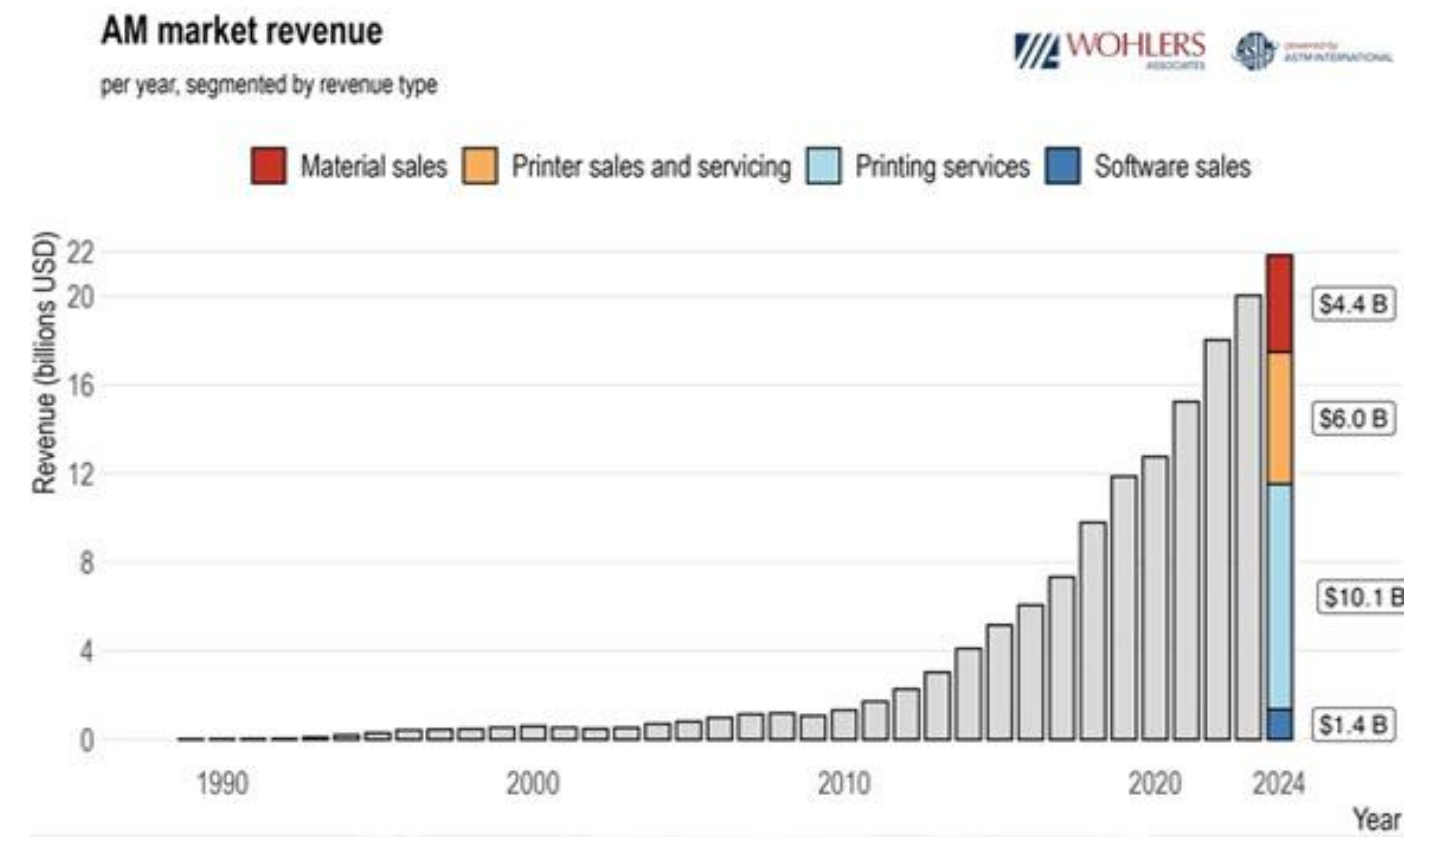
\includegraphics[width=0.5\textwidth]{assets/economischegroei.png}
  \caption{Economische groei additive manufacturing}
  \label{fig:economischegroei.png}
 \end{figure}
Vooral omdat dit prototyping zeer makkelijk maakt en goedkoop is.
\subsection{Application levels → hoe wordt het gebruikt?}
Er wordt een hoofdonderverdeling gemaakt tussen 2 toepassingsniveaus: \textbf{Rapid Prototyping} en \textbf{Rapid Manufacturing}.
\begin{figure}[H]
  \centering
  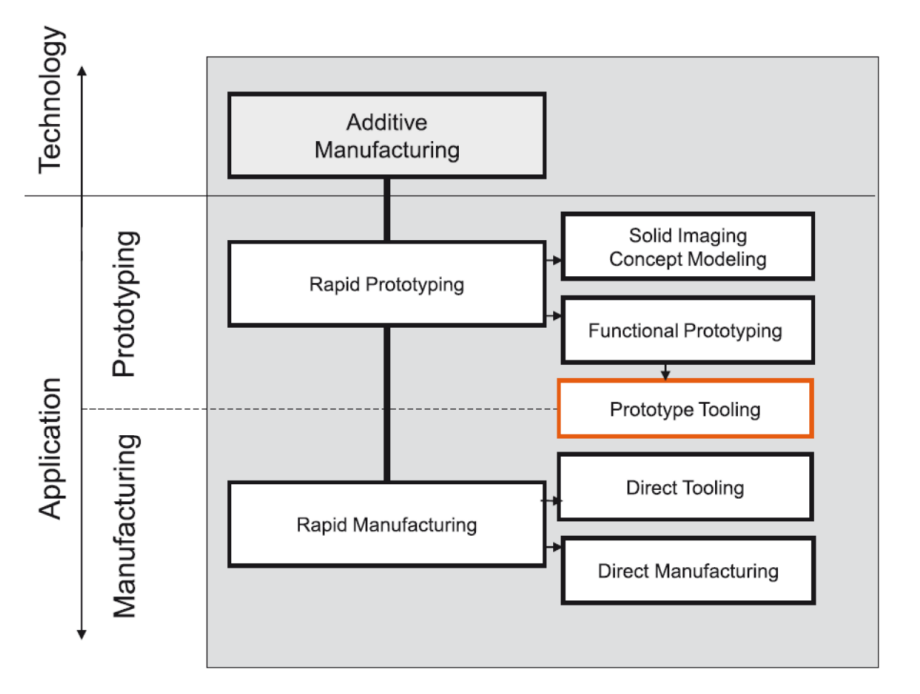
\includegraphics[width=0.6\textwidth]{assets/hoofdniveaus.png}
  \caption{Hoofdniveaus}
  \label{fig:hoofdniveaus.png}
 \end{figure}
\subsubsection{Rapid Prototyping}
Dit is het snel ontwikkelen van prototypes, het bevat ook nog subcategorieën zoals :
\begin{itemize}
   \item \textbf{Solid imaging and concept modeling: }Dit wordt gebruikt voor visuele conceptmodellen. De slide toont als voorbeeld een geprint schaalmodel van een motor.
   \item \textbf{Functional prototyping: }Dit wordt gebruikt voor het testen van de functionaliteit van een ontwerp (werkende prototype). De slide toont als voorbeeld een geprint model van een vliegtuig dat wordt getest in een windtunnel.
\end{itemize}
\subsubsection{Rapid Manufacturing}
Dit is het snel produceren van eindproducten, het bevat ook nog subcategorieën zoals :
\begin{itemize}
    \item \textbf{Direct manufacturing: }Het direct printen van functionele eindproducten. De voorbeelden hierbij zijn een driedelige tandheelkundige brug en een scharnier voor de motorkap van een vliegtuig (die vergeleken wordt met een conventioneel gemaakte versie)
    \item \textbf{Direct tooling:} Het direct printen van productiegereedschap, zoals een stalen matrijs die gebruikt wordt voor blaasvormen (blow molding)
\end{itemize}
\subsubsection{Prototype tooling}
Dit is nog een tussenniveau, dit is het maken van tijdelijk gereedschap voor de prototypefase, geïllustreerd met een matrijs voor de zool van een rubberen laars.
\subsection{Prototyping}
Dit is het snel ontwikkelen van prototypes, waarom? Het heeft 5 hoofddoelen en voordelen:
(de proff ging snel over deze slides)
\begin{itemize}
  \item \textbf{Risicoreductie:} Een prototype helpt om te controleren of het model aan de verwachtingen voldoet, visueel kan ook al nagekeken worden, of de klant het goed vind ook, functies kunnen getest worden (en limieten), dit bespaart ook allemaal grote investeringen voor we naar het echte product gaan, dus willen we op voorrand zeker zijn dat het product goed is.
  \item \textbf{Kostenreductie:} Door prototyping kan het ontwerp vroegtijdig geoptimaliseerd worden om zo fouten op te sporen en de haalbaarheid te testen. Additive manufacturing is hierbij voordeliger omdat traditionele modelbouw vaak arbeidsintensiever en duurder is, en minder nauwkeurige of levensechte resultaten oplevert. Dit is ook een \textbf{itereerbaar} proces.
  \item \textbf{Kortere 'Time to Market':} Versnelt de productontwikkeling waardoor je sneller de markt op kunt en de concurrentie voor blijft.
  \item \textbf{Ondersteuning van verkoop en marketing:} Een tastbaar model is direct inzetbaar voor klantpresentaties, testpubliek en fotoshoots.
  \item \textbf{Communicatie:} Een fysiek prototype praat makkelijker en verbetert de afstemming tussen teams, klanten en leveranciers.
\end{itemize}
\subsection{Manufacturing-Customization (Productie op maat)}
Hier is tegenwoordig extra vraag naar, ook naar de massaproductie er van, vooral in de \textbf{medische sector} (hoortoestellen, tandheelkundige toepassingen, op maat gemaakte implantaten en medisch gereedschap zoals chirurgische geleiders (surgical guides)
.) en de \textbf{industriele sector} (Naast de medische sector is er ook sprake van maatwerk in de bredere industrie. Bij deze toepassingen wordt op de slides specifiek verwezen naar de bedrijven P2L, Materialise en Zagato als praktijkvoorbeelden
.)
\begin{figure}[H]
  \centering
  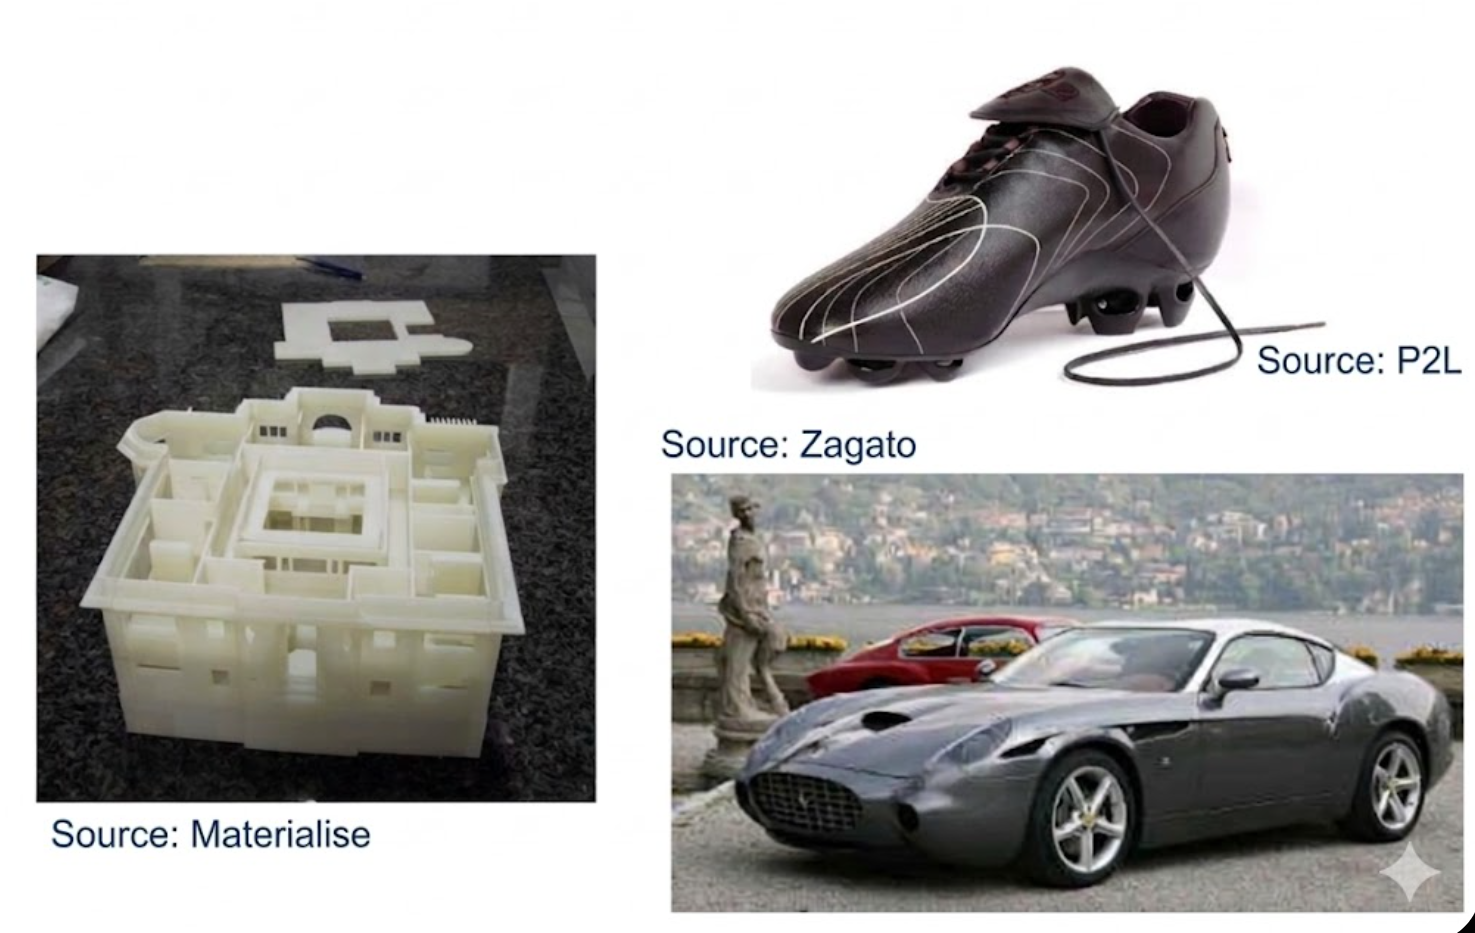
\includegraphics[width=0.6\textwidth]{assets/industriesector.png}
  \caption{Voorbeelden industriesector}
  \label{fig:industriesector.png}
 \end{figure}
\subsection{Manufacturing - Low volume series (Kleine series)}
We moeten natuurlijk weten dat niet alles zal worden ge 3D-print, voor kleine hoeveelheden kan het voordelig zijn, in de toekomst zal het waarschijnlijk goedkoper worden en meer en meer voordeliger worden dan andere productietechnieken. De optimale techniek vinden hangt dus af van de beschikbare technologie en de complexiteit van het ontwerp.
\begin{figure}[H]
  \centering
  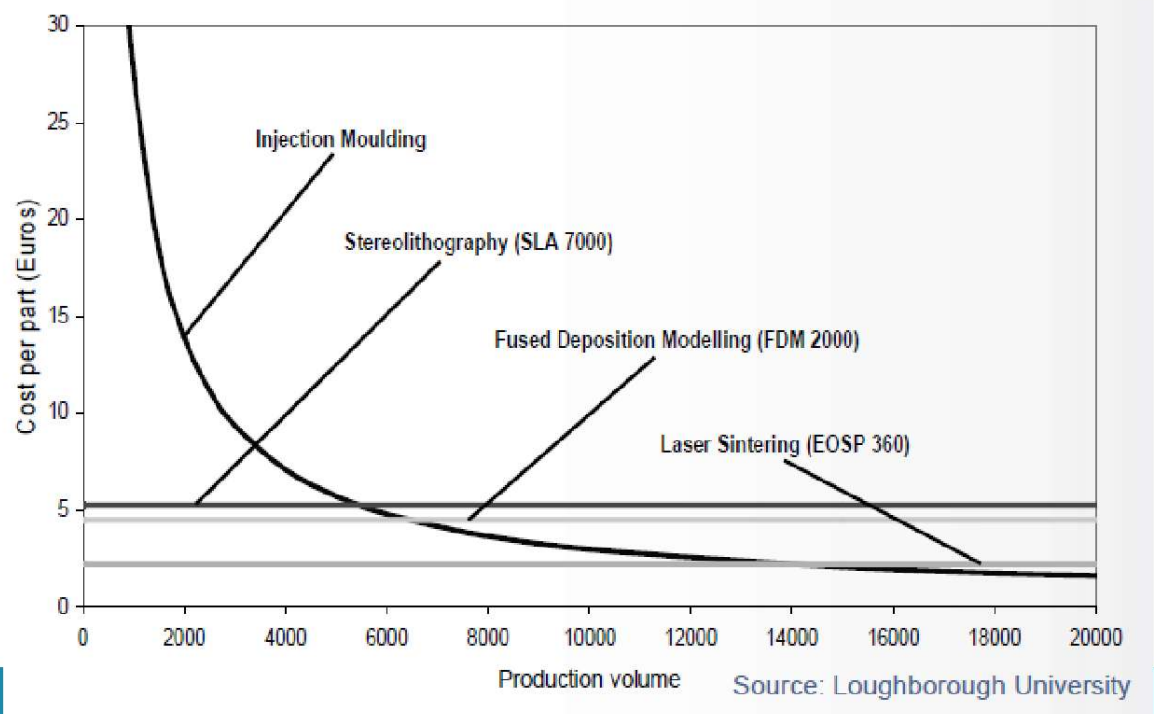
\includegraphics[width=0.6\textwidth]{assets/grafiekAM.png}
  \caption{kostprijs per onderdeel in functie van het productievolume}
  \label{fig:grafiekAM.png}
 \end{figure}
De foto toont een grafiek met de kostprijs per onderdeel in functie van het productievolume, waarbij spuitgieten (Injection Moulding) wordt vergeleken met AM-technieken (SLA, FDM, SLS)
. De proff verklaart hierbij dat de kost van 3D-printen vrijwel onafhankelijk is van het aantal stuks (een nagenoeg horizontale dalende lijn), waardoor er een omslagpunt is en 3D-printen voordeliger is voor weinig stuks.
Als je van een product een grote hoeveelheid nodig hebt, is het voordeliger om een matrijs te maken en te spuitgieten, maar als je maar een paar stuks nodig hebt, is 3D-printen voordeliger omdat er geen dure matrijs nodig is.
Met 3D-printen kan je ook 'geintegreerde producten' printen, dit betekent dat assembly's in 1 geheel geprint kunnen worden, iets wat met spuitgieten bevoorbeeld niet kan, het is dus niet nodig meer om verschillende onderdelen te maken en deze dan samen te voegen.
Met 3D printen kan je dus complexe geometrieën maken en dus als je slim bent kan dit je materiaal en gewicht besparen, dit is vooral belangrijk in de luchtvaartindustrie, zie foto :
\begin{figure}[H]
  \centering
  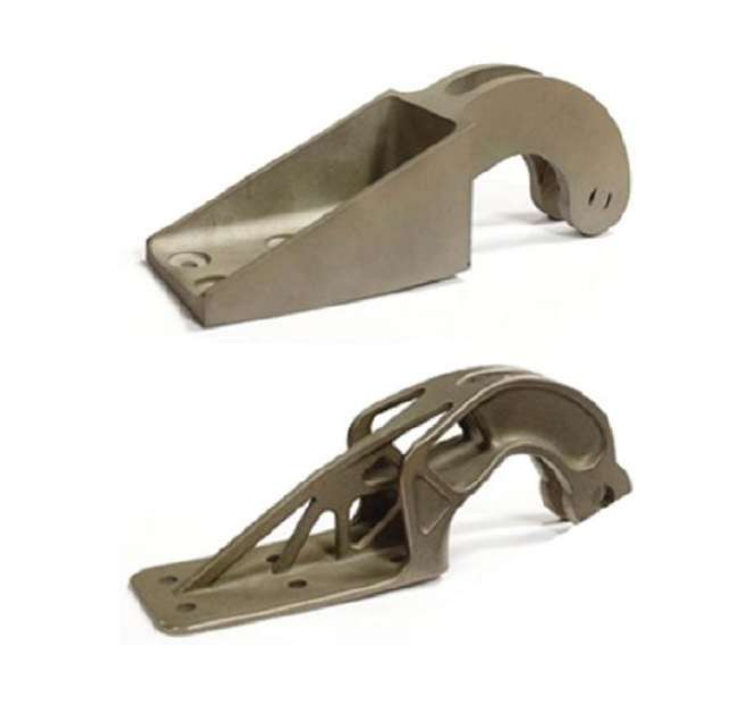
\includegraphics[width=0.4\textwidth]{assets/lichtgewichtAM.png}
  \caption{Zwaardere identieke functie onderdeel vanboven en lichtere complexere versie vanonder, gemaakt met AM}
  \label{fig:lichtgewichtAM.png}
 \end{figure}
\subsection{AM workflow (Proces van AM)}
Nu gaan we het stappenplan om van een digitaal ontwerp tot een fysiek geprint en nabewerkt product te gaan beschrijven. Dit heeft verschillende fases en concepten.
\begin{figure}[H]
  \centering
  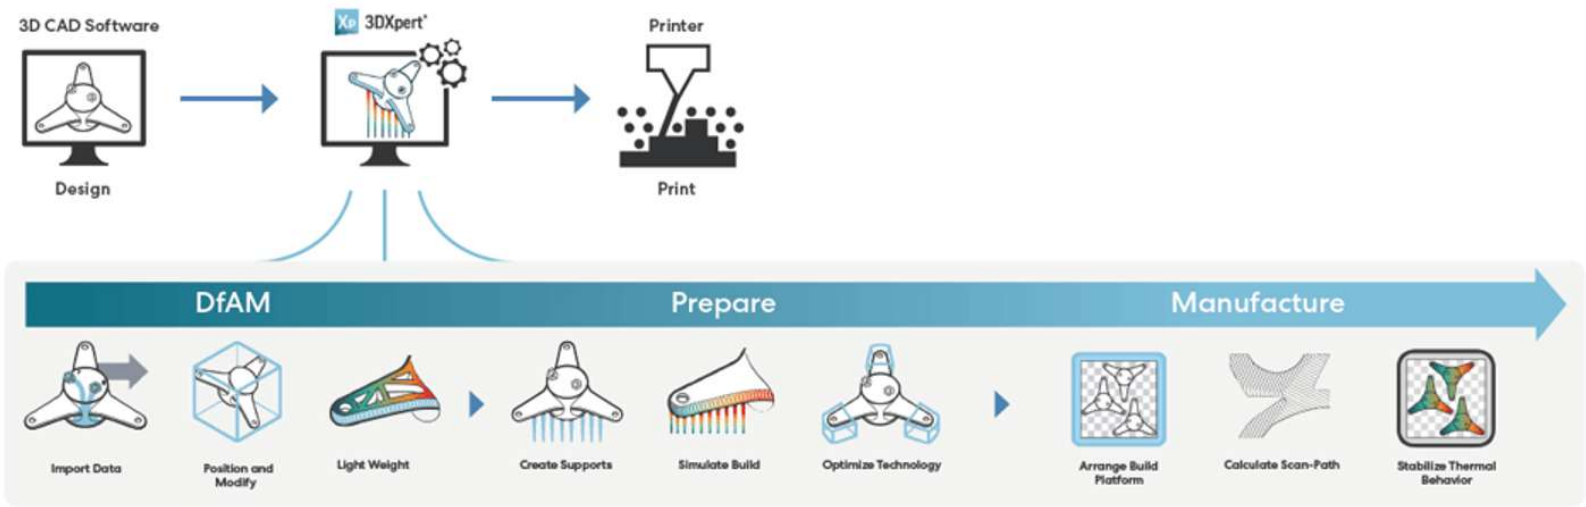
\includegraphics[width=0.9\textwidth]{assets/AMworkflow.png}
  \caption{AM workflow}
  \label{fig:AMworkflow.png}
 \end{figure}
\subsubsection{Design (Ontwerp) for Additive Manufacturing (DfAM)}
Dit is eigelijk de eerste fase, Het proces start met 3D CAD-software. Vaak wordt dit geëxporteerd als een \textbf{.STL-bestand}, wat enkel de buitencontouren (driehoekjes) van het model beschrijft. Betere alternatieven zijn \textbf{.3MF en .AMF}, omdat deze ook interne structuren, materiaalkeuze en kleuren kunnen bevatten, je hebt ook nog \textbf{.VRML}, dit is iets voor in virtual reality. Tijdens DfAM (Design for AM) wordt het model geanalyseerd en geoptimaliseerd, bijvoorbeeld door het lichter te maken ('light weighting') via roosterstructuren en het optimaal te positioneren voor de print.
\subsubsection{Prepare (voorbereiden)}
Deze fase gaat over het toevoegen van steunstructuren (dit zijn 'supports') en dat deze cruciaal zijn om overhangende delen te printen en om overtollige warmte af te voeren. De juiste printinstellingen zijn ook belangrijk, ontwerpoptimalisatie en printinstellingen beïnvloeden elkaar sterk en gebeuren vaak gelijktijdig.
\subsubsection{Manufacture (productie)}
Productie willen we natuurlijk zo vlot mogelijk of zo efficiënt mogelijk laten verlopen, concepten die hiermee kunnen helpen/te maken hebben zijn:
\begin{itemize}
  \item \textbf{Nesting:} Het efficiënt plaatsen van meerdere onderdelen op het printbed om materiaal en tijd te besparen. Het is vooral de laaghoogte die je minimaal wilt houden eigelijk, zie foto. Dit wordt vooral toegepast bij polymeer SLS (Selective Laser Sintering), omdat het ongesmolten poederbed hier als natuurlijke ondersteuning dient en er geen geprinte steunstructuren nodig zijn.
  \begin{figure}[H]
    \centering
    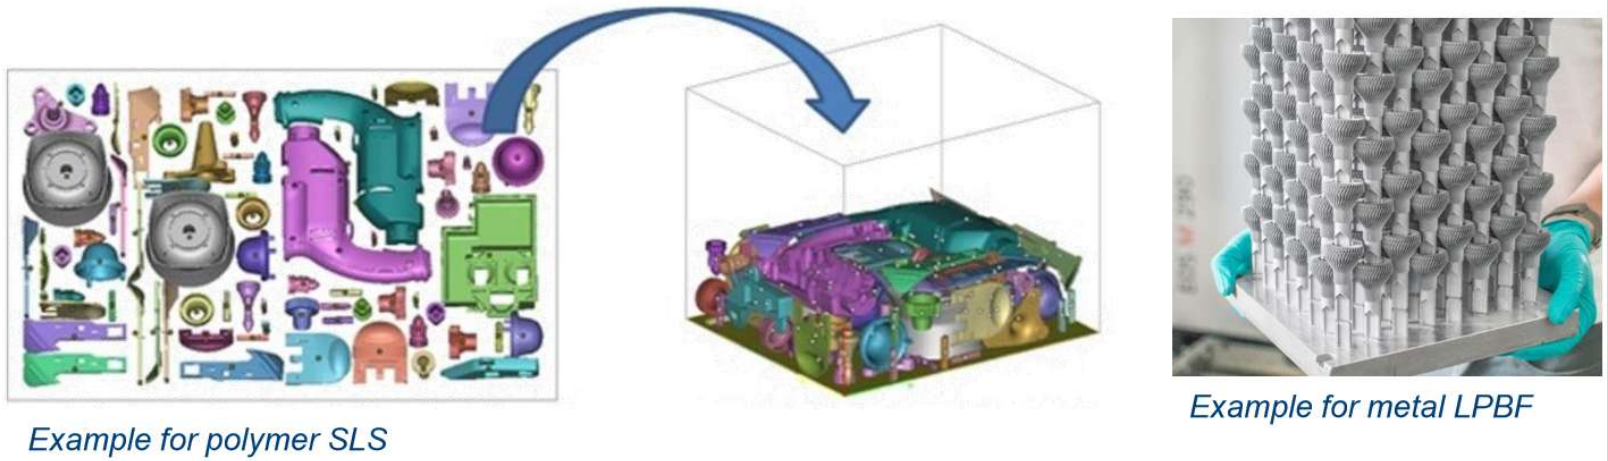
\includegraphics[width=0.8\textwidth]{assets/nesting.png}
    \caption{Nesting}
    \label{fig:nesting.png}
   \end{figure}
  \item \textbf{Slicing \& Scan-pad:} Het model wordt in dunne horizontale laagjes gesneden ('slicing'). Vervolgens wordt de scanstrategie (hatching) bepaald: hoe de laser het materiaal per laag gaat consolideren (bijvoorbeeld met lijntjes in één of meerdere richtingen). (m.a.w. slicing van het model vertaalt het cad-model naar de machine-instructies voor de printer omdat deze laag per laag print)
  \begin{figure}[H]
    \centering
    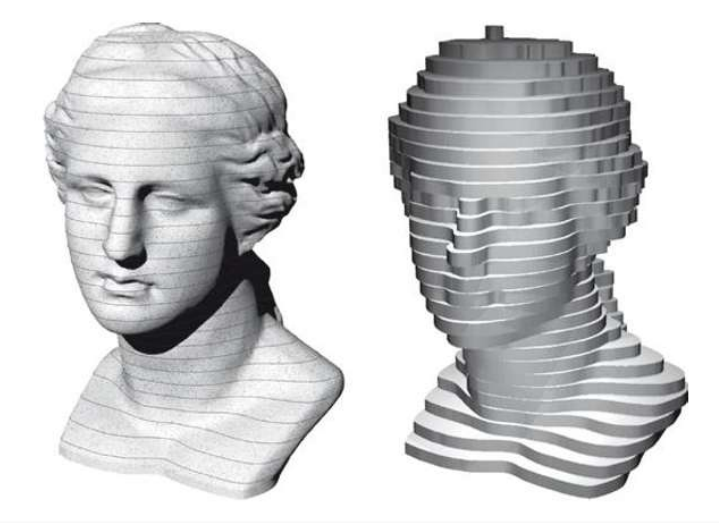
\includegraphics[width=0.4\textwidth]{assets/slicing.png}
    \caption{Sliced model (wel heel weinig lagen, wordt dus een kleine print)}
    \label{fig:slicing.png}
   \end{figure}
  \begin{figure}[H]
    \centering
    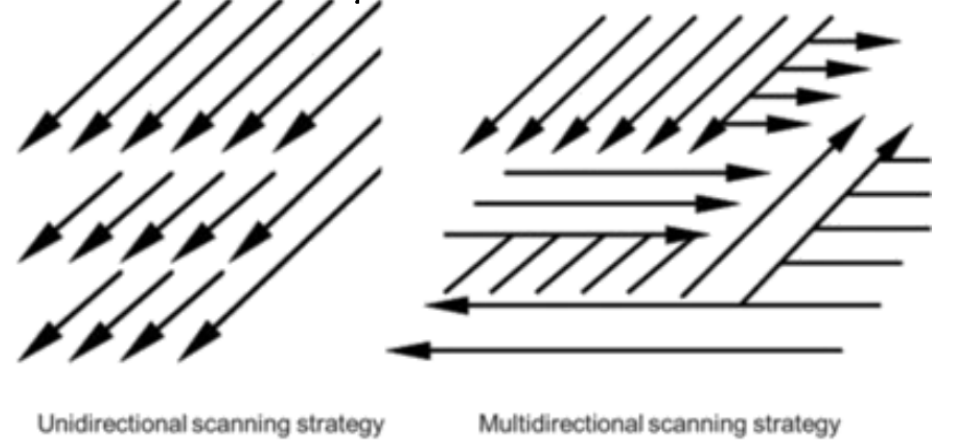
\includegraphics[width=0.7\textwidth]{assets/scanstrategien.png}
    \caption{Scanstrategien}
    \label{fig:scanstrategien.png}
   \end{figure}
  De figuur hierboven toont \textbf{unidirectionele scanstrategie}, hierbij trekt de laser eigelijk lijntjes in één richting om een vlak te vullen. Ook zien we \textbf{multidirectionele scanstrategie}, de laser scant dan in meerdere richtingen, bijvoorbeeld door lijnen in verschillende hoeken over het vlak te trekken. Er is ook nog \textbf{'Island scanning'}, hierbij wordt het te printen vlak opgedeeld in kleinere secties of "eilandjes", die vervolgens per stuk door de laser worden ingescand.
  Naast het patroon binnen één enkele laag, moet men ook kiezen hoe de scanstrategie zich gedraagt van de ene laag op de andere. Vaak wordt het patroon bij elke nieuwe laag bijvoorbeeld een beetje gedraaid, wat de sterkte van het onderdeel ten goede komt.
\item \textbf{Energiedensiteit:} De energiedensiteit (E) is 1 van de belangrijkste parameters bij laserbedgestuurde poeder-technieken, het geeft aan hoeveel laserenergie er per volume-eenheid aan het materiaal wordt toegevoegd om het poeder te smelten. Deze éénheid wordt als volgt berekent:
  \frm{Energiedensiteit}{E = \frac{P}{v \cdot h \cdot t}}
  {met \sym{P}{Vermogen}{\si{W}} \sym{v}{Scansnelheid}{\si{m/s}} \sym{h}{Hatchafstand}{\si{m}} \sym{t}{Laagdikte}{\si{m}}}
\begin{figure}[H]
  \centering
  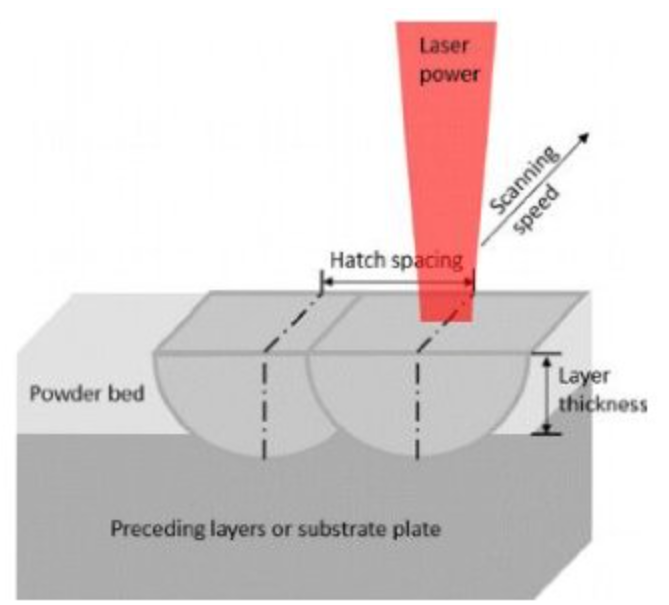
\includegraphics[width=0.5\textwidth]{assets/energiedensiteit.png}
  \caption{Vizualisatie van energiedensiteit}
  \label{fig:energiedensiteit.png}
 \end{figure}
De energiedensiteit bij lasers hangt af van vier parameters: het vermogen (P), de scansnelheid (v), de hatch spacing (h) en de laagdikte (t). Een hoger vermogen zorgt voor meer energie-inbreng, terwijl een hogere scansnelheid net minder energie per plaats geeft. Als de hatch spacing groter wordt, wordt de energie over een breder gebied verdeeld, en een grotere laagdikte betekent dat de energie over meer materiaal wordt verspreid.
\begin{warningbox}[Let op!]
De ingestelde laagdikte (t) mag je niet verwarren met de smeltbaddiepte: de laser smelt altijd dieper dan één laag, zodat ook een deel van de vorige laag mee smelt en beide lagen goed aan elkaar hechten. De laser moet namelijk niet alleen de nieuwe laag poeder smelten, maar ook een stukje van de reeds geprinte laag daaronder, zodat beide lagen goed aan elkaar vastsmelten en consolideren.
\end{warningbox}
\subsubsection{Finishing (nabewerking)}
Als laatste fase is er de nabewerking, dit is het verwijderen van de supports, het gladmaken van het oppervlak, eventueel warmtebehandelingen om de mechanische eigenschappen te verbeteren, en andere post-processing stappen zoals schilderen of coaten. Oppervlaktenabewerking is vaak toepasbaar met technieken zoals zandstralen, polijsten, mechanisch bewerken, \dots
\begin{figure}[H]
  \centering
  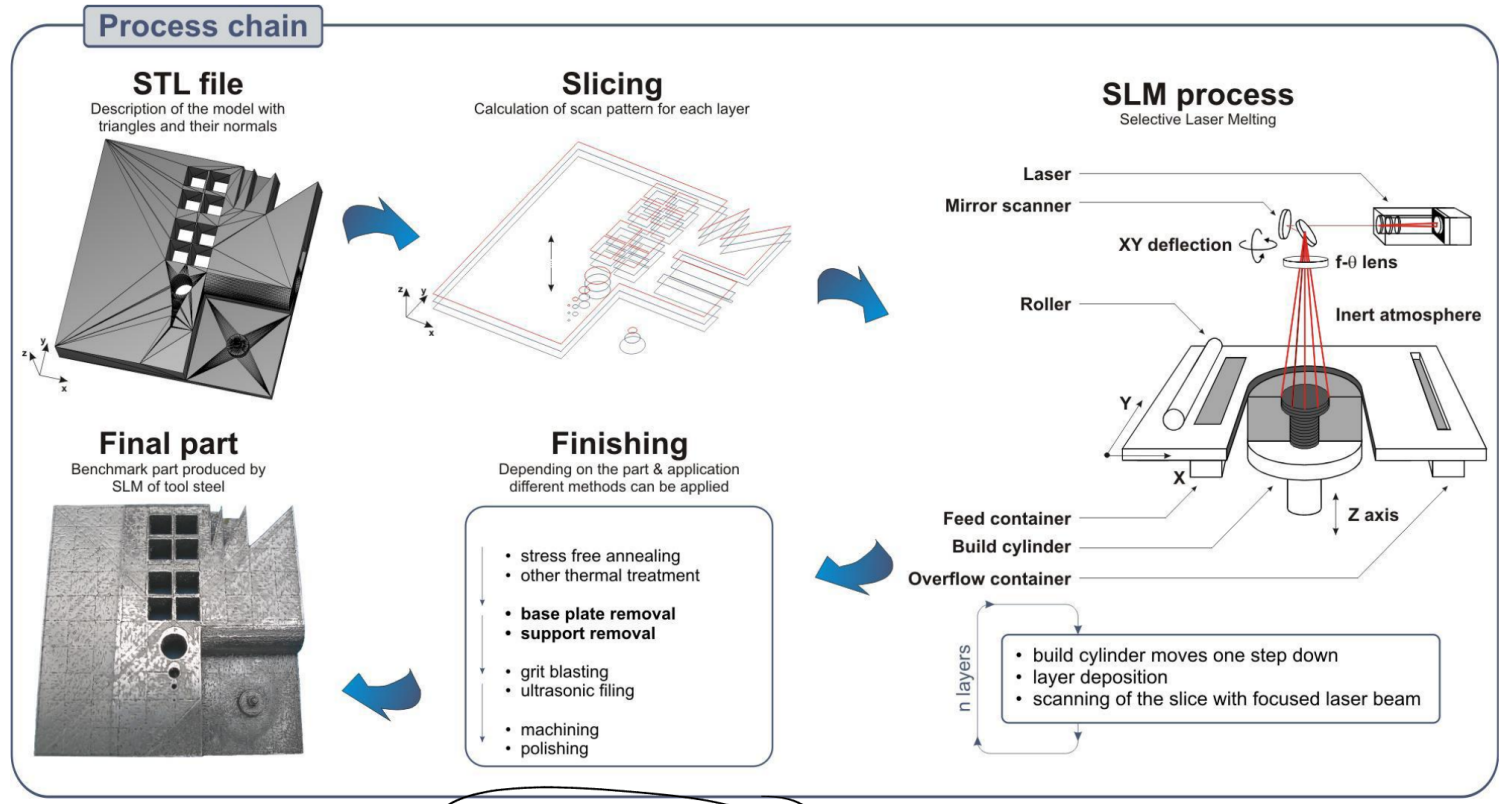
\includegraphics[width=1\textwidth]{assets/AMworkflowsamenvattend.png}
  \caption{Samenvattende figuur van de AM workflow}
  \label{fig:AMworkflowsamenvattend.png}
 \end{figure}
\end{itemize}
\subsection{AM Strengths (Voordelen van 3D printen)}
Dit is vanzelfsprekend, er zijn 5 grote voordelen van additive manufacturing:
\begin{itemize}
  \item \textbf{Snelheid:} Hoewel het printen zelf heel traag is, is het hele proces ervoor (en erna) veel sneller dan traditionele productiemethoden, Je kunt bijvoorbeeld in de middag een CAD-model krijgen, het in de namiddag simuleren en instellen, en 's avonds direct beginnen met printen, dit versnelt en automatiseert de prototypingfase, verkort de herontwerp-cyclus en de time-to-market, en bespaart assemblagetijd doordat functionaliteiten al in één onderdeel geïntegreerd kunnen worden.
  \item \textbf{Ontwerpvrijheid (Freedom of Design):} Men heeft enorm veel vrijheid tijdens het ontwerpen, waardoor "onmogelijke" ontwerpen nu wel mogelijk worden. Een enorm voordeel hierbij is dat een hoge complexiteit van het ontwerp vrijwel geen invloed heeft op de kostprijs.
  \item \textbf{Lagere kosten voor kleine series:} Doordat er sprake is van minder arbeidsintensieve handelingen en veel lagere investeringskosten in vergelijking met traditionele methodes, is AM ideaal voor kleine oplages. De proff zegt dat dit rendabel kan zijn voor series tot zo'n 10.000 à 50.000 stuks per jaar.
  \item \textbf{Flexibiliteit:} Dit gaat hier terug over die itereerbaarheid, je kan snel aanpassingen maken in het ontwerp en direct opnieuw printen, dit is vooral handig in de prototypingfase.
  \item \textbf{Just In Time (JIT) productie:} Dit zorgt voor ware "on demand" productie (produceren op het moment dat er vraag is). Hierdoor kunnen de opslagkosten aanzienlijk worden verlaagd, omdat men reserveonderdelen niet meer jarenlang fysiek in een magazijn hoeft op te slaan, maar simpelweg print wanneer ze nodig zijn.
\end{itemize}
\subsection{AM Limitations (Beperkingen van 3D printen)}
Natuurlijk zijn er ook beperkingen, dit zijn de belangrijkste:
\begin{itemize}
 \item \textbf{Nauwkeurigheid:} Dit wordt sterk bepaald door de laagdikte, door het laagsgewijs opbouwen ontstaat er op schuinve vlakken een zichtbaar 'staircase effect'.  Ook kunnen we ongesmolten poederdeeltjes hebben die aan het werkstuk blijven kleven bij poederbedtechnieken, omdat de oppervlaktekwaliteit hierdoor vaak niet optimaal is, zijn er in veel gevallen nog nabewerkingsstappen nodig, ook wordt de algemene procescontrole als een beperking gezien.
 \begin{figure}[H]
   \centering
   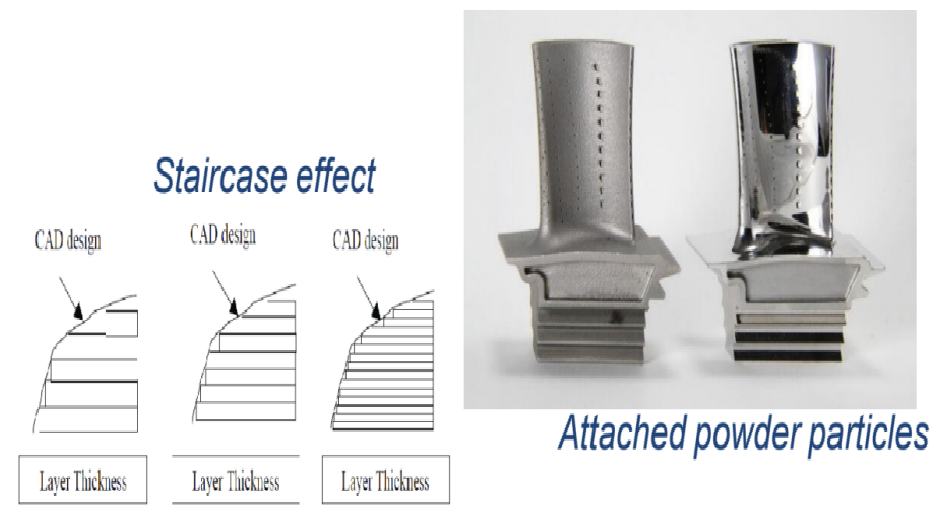
\includegraphics[width=0.6\textwidth]{assets/SCAPP.png}
   \caption{Staircase effect en ongesmolten poederdeeltjes bij poederbedtechnieken}
   \label{fig:SCAPP.png}
  \end{figure}
 \item \textbf{Hogere kosten voor grotere series:} AM kent hogere operationele kosten. Hierdoor is het proces te duur en niet rendabel voor massaproductie (high volume series) in vergelijking met traditionele technieken.
 \item \textbf{Materialen:} Er zijn grenzen aan de mechanische eigenschappen, de beschikbaarheid en de kostprijs van materialen. Ook moeten materialen in een heel specifieke, verwerkbare vorm beschikbaar zijn om de printer te kunnen voeden, zoals draden op een spoel of perfect ronde poederkorrels, een probleem is dat niet alle bestaande metaallegeringen tot dit soort printbare poeders verwerkt kan worden.
\end{itemize}
Hiermee kan al geconcludeerd worden dat AM conventionele productietechnieken niet zal vervangen, maar het echter wel een enorm interessante piste voor bepaalde toepassingen kan zijn. Het geeft meer mogelijkheden.
\newpage
\subsection{Ontwerpen voor AM}
\subsubsection{Ontwerpregels}
Net zoals je bij het traditioneel frezen rekening moet houden met de vorm van je gereedschap (zoals het afronden van hoeken), heeft 3D-printen zijn eigen specifieke regels.
\begin{itemize}
 \item \textbf{Minimale afmetingen:} De kleinste details die je kan printen, worden direct beperkt door de breedte van de laserstraal (single scan width).
 \item \textbf{Overhangende delen:} Als je al ooit ge 3D-print hebt, weet je waar ik het over heb, oppervlaktes van overhangende delen zijn vaker van slechtere kwaliteit omdat er steunstructuren nodig zijn, geometrie slim aanpassen of printoriëntatie variëren kan dit voorkomen of het probleem verminderen.
 \item \textbf{Ingesloten holtes:} Bij processen die met een poederbed werken moet je hiermee oppassen, want het ongesmolten poeder raakt dan permanent opgesloten in het binnenste van je werkstuk.
 \item \textbf{Steunstructuren:} Deze wil je dus zo veel mogelijk vermijden, achteraf moet je deze verwijderen, ze spelen niet alleen een rol in stabiliteit maar ook in het wegleiden van warmte en tegengaan van thermische vervormingen.
\end{itemize}
\subsubsection{Nieuwe ontwerpmogelijkheden}
Dankzij de grote ontwerpvrijheid van AM kunnen we ontwerpen maken die met conventionele technieken onmogelijk zijn om te maken. Honinggraat- of roosterstructuren zijn een mooi voorbeeld, deze worden gebruikt omdat ze lichtgewicht zijn, dit wordt gemaakt met topologische optimalisatie, je vertrekt hierbij van een bestaand, massief ontwerp dat wordt geanalyseerd door software zodat de software dan het 'dode gewicht' verwijderd op plekken waar het materiaal niet structureel belast wordt. Dit geeft je 1 optimale vorm die veel lichter is, maar toch dezelfde vereiste sterkte en stijfheid behoudt. Je hebt ook nog \textbf{generatief ontwerpen}, hier geef je de software randvoorwaarden (constraints), hiermee gaat de computer zelf verschillende ontwerpopties bedenken die dan aan die eisen voldoen, opvallend is dat deze vaak een vloeiende organische vormgeving hebben die ons doet denken aan structuren uit de natuur.
\begin{figure}[H]
  \centering
  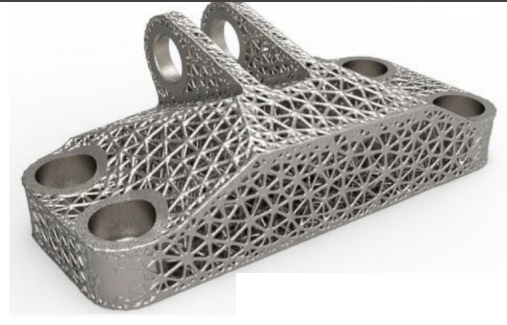
\includegraphics[width=0.4\textwidth]{assets/honinggraat.png}
  \caption{Honinggraat- of roosterstructuren}
  \label{fig:honinggraat.png}
 \end{figure}
\subsection{AM process categories (AM procescategorieën)}
De volgende figuur toont de 7 hoofdcategorieën van 3D-printtechnieken (volgens de ISO/ASTM standaard):
\begin{figure}[H]
  \centering
  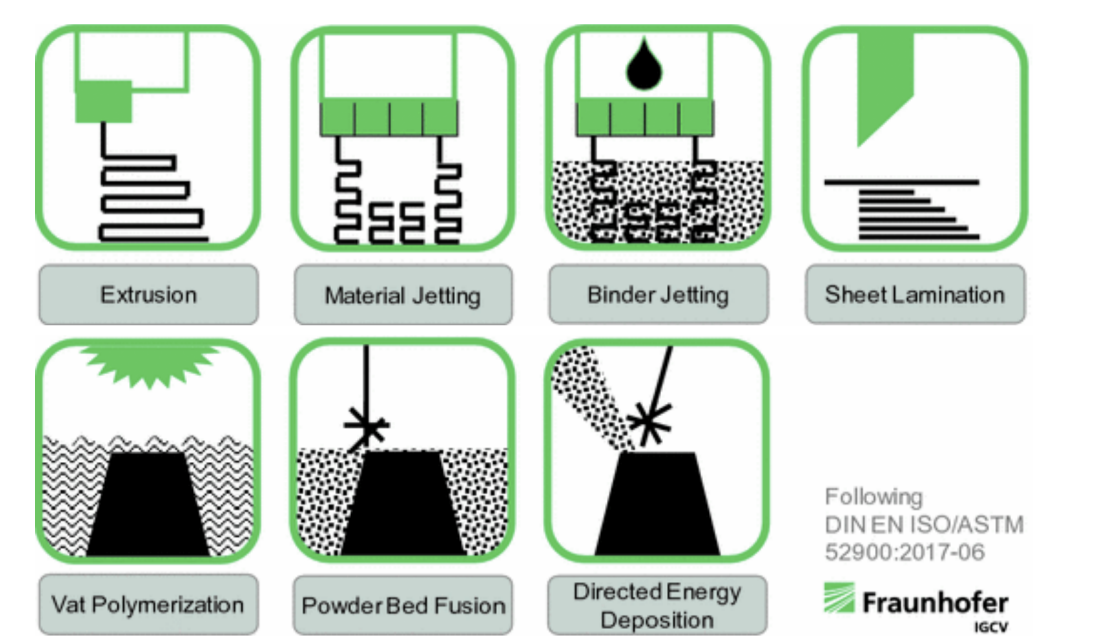
\includegraphics[width=0.8\textwidth]{assets/hoofdcategorienAM.png}
  \caption{7 hoofdcategorieën van 3D-printtechnieken volgens ISO/ASTM standaard}
  \label{fig:hoofdcategorienAM.png}
 \end{figure}
Alle bestaande printtechnieken zijn van elkaar te onderscheiden op basis van 2 belangrijke eigenschappen:
\begin{itemize}
 \item \textbf{Materiaaltoevoer:} Hoe wordt het materiaal in de machine gebracht? (kan poederbed, draad of vat met vloeistof zijn)
 \item \textbf{Consolidatiemechaniscme:} Hoe zorg je ervoor dat het materiaal uithardt of aan elkaar plakt? (bvb. door te smelten, via lijm of via UV-licht)
\end{itemize}
Dan bezien we tot slot kort de 7 categorieën:
\subsubsection{Material Extrusion}
Hier wordt een thermoplastisch polymeer in de vorm van een draad (filament) of als korrels (pellets) aangevoerd. Het materiaal wordt door een verwarmde nozzle getrokken of geduwd waardoor het smelt en vervolgens laagsgewijs wordt afgezet op het bed (bouwplatform). Dit staat bekend als Fused Filament Fabrication of Fused Deposition Modeling. Meestal zijn de materialen PLA en ABS of andere polymeer composieten, een nieuwe ontwikkeling is het gebruik van polymeerdraden die metaal- of keramiekdeeltjes bevatten. Daar dient het plastic dan als tijdelijk bindmiddel, na het printen is wel een extra bewerkingsstap nodig om het polymeer weg te branden en de metaaldeeltjes aan elkaar te sinteren.
\begin{figure}[H]
  \centering
  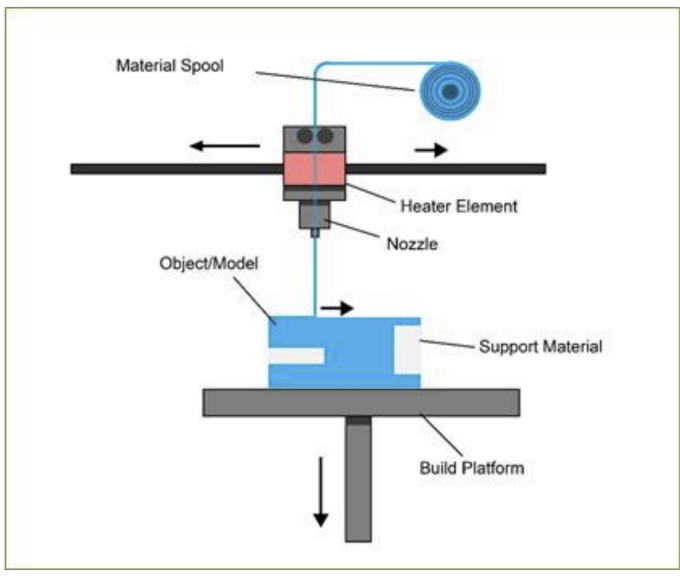
\includegraphics[width=0.5\textwidth]{assets/MATE.png}
  \caption{Material Extrusion (FDM/FFF)}
  \label{fig:MATE.png}
 \end{figure}
Dit is een erg goedkoop en makkelijk proces (voor hobby 3D-printers) maar het heeft ruwere oppervlaktekwaliteit en matige mechanische eigenschappen, dit is omdat de draad eigelijk nooit 100\% smelt, wat resulteert in een werkstuk met een deel aan porositeit wat de sterkte vermindert.
\subsubsection{Material jetting}
Hier wordt vloeibare 'hars' (liquid resin) druppelsgewijs of continu uit een printkop gespoten, zodra die druppels landen worden ze uitgehard met behulp van UV-licht. Typisch gebruikt men polymeren (UV-uithardende harsen) en composieten (vloeibare inkt met metaal-of keramiekdeeltjes), er bestaan ook technieken voor metalen met een laag smeltpunt zoals aluminium (liquid metal jetting). Deze techniek biedt enorm veel voordelen, het heeft extreem hoge precisie en laat toe om verschillende materialen en zelfs kleuren (via inkt) toe te voegen in 1 print. Een nadeel is wel het relatief klein bouwvolume en de instabiliteit van het product over tijd, hiermee bedoelen we sinds dat het materiaal specifiek reageert op UV-licht dat het buiten, waar de zon is, langzaam aan ook verder blijven reageren en bvb. verkleuren. Dit is een prachtige techniek voor het maken van hoogwaardige meerkleurige visuele modellen.
\begin{figure}[H]
  \centering
  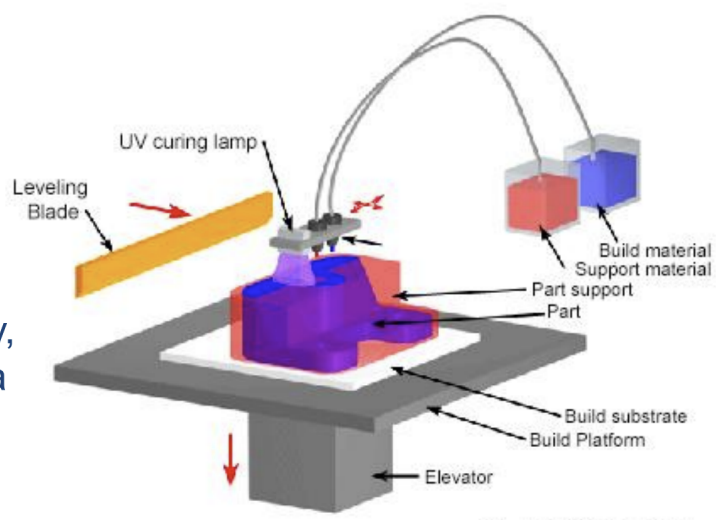
\includegraphics[width=0.5\textwidth]{assets/materialjetting.png}
  \caption{Material jetting (UV-uithardende harsen)}
  \label{fig:materialjetting.png}
 \end{figure}
\begin{figure}[H]
  \centering
  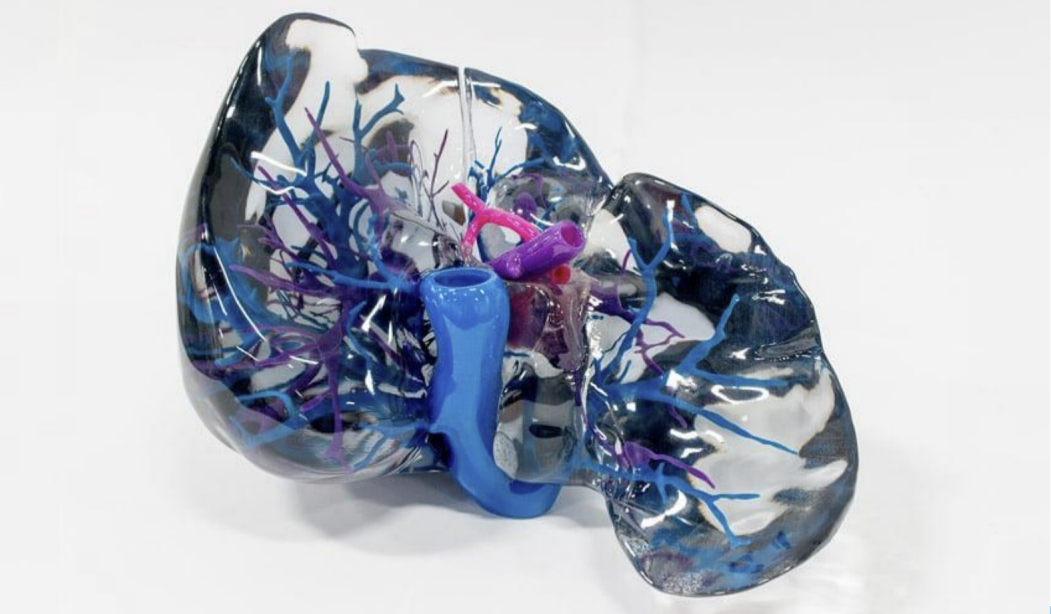
\includegraphics[width=0.5\textwidth]{assets/printvoorbeeldmatjet.png}
  \caption{Voorbeeld van een material jetting print}
  \label{fig:printvoorbeeldmatjet.png}
 \end{figure}
\subsubsection{Binder jetting}
Dit is een techniek dat ook laagsgewijs werkt maar hier met een poederbed als structureel materiaal, een printkop spuit druppels van een vloeibaar bindmiddel (liquid binder) op dat poeder, op die plakken gaat het materiaal moeten samenplakken, daarna wordt er een nieuwe laag poeder over verdeeld en herhaalt het proces zich. Je hebt het standaard binder jetting en je hebt multi jet fusion (van HP), dit is een extreem snel proces want het gebruikt honderden van die jetting nozzels (printmondjes). Het materiaal hier kan vanalles zijn, typisch wordt zand of PMMA (polymeer) gebruikt, nu kan het sinds recent ook met metaalpoeders, dit vereist wel een extra stap, na het printen moet het bindmiddel eruit gebrand worden (bespraken we eerder ook) en daarna het metaal gesinterd, dit is voordelig want je vermijd restspanningen in grote metalen stukken. Dit proces is ook heel snel en je kan grote kleurrijke stukken maken, er zijn ook geen supports nodig, nadeel is wel dat de oppervlaktekwaliteit niet zo goed is en het product heeft matige mechanische eigenschappen. Wordt vooral gebruikt om zandmallen voor metaalgieterijen te maken.
\begin{figure}[H]
  \centering
  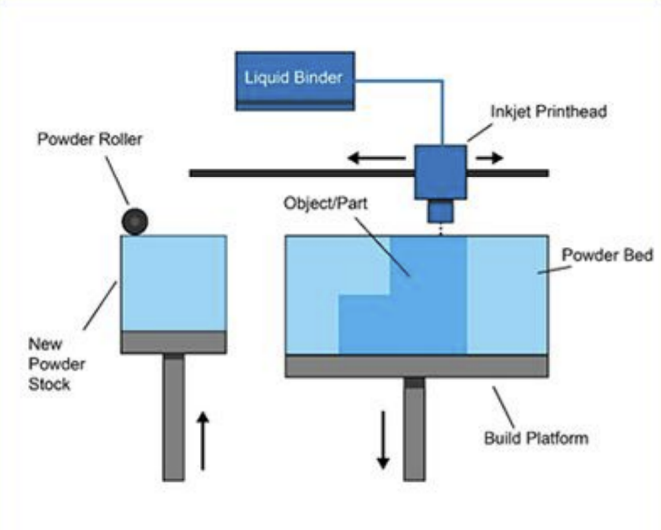
\includegraphics[width=0.5\textwidth]{assets/binderjetting.png}
  \caption{Binder jetting}
  \label{fig:binderjetting.png}
 \end{figure}
\newpage
\subsubsection{Sheet lamination}
Vergeleken met de rest is dit eigelijk een minder 3D-printtechniek, het wordt ook niet zo vaak gebruikt, er wordt hier vertrokken van een plaatmateriaal of vellen, die worden op elkaar gestapeld en gelast of gelijmd. Het overtollig materiaal (de delen van de platen die je nie nodig hebt) moet daarna nog fysiek weggesneden worden. Ultrasonic AM en Laminated Object Manufacturing (LOM) zijn bekende technieken hierbij. Hier kan echt elk soort plaatmetaal gebruikt worden, composieten ook of gewoon papier met lijm kan ook. Het is een heel makkelijk en snel proces, gekleurde stukken kan ook maar het heeft enorm veel waste door dat wegsnijden en eigelijk is de materiaalkeuze een beetje beperkt en de materiaaleigenschappen zijn matig. Wordt gebruikt om bvb. 3D topografische kaarten te maken.
\begin{figure}[H]
  \centering
  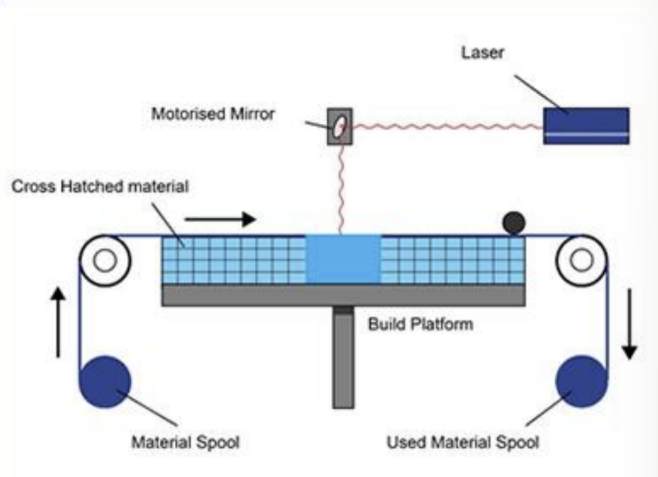
\includegraphics[width=0.5\textwidth]{assets/sheetlamination.png}
  \caption{Sheet lamination}
  \label{fig:sheetlamination.png}
 \end{figure}
\subsubsection{Vat polymerization}
Het bouwoppervlak bevindt zich hier in een vat (bad) gevuld met vloeibaar 'fotopolymeer' (resin/hars). Een laser of UV-lamp hardt het vloeibaar materiaal laag per laag selectief uit, als een laag is uitgehard, zakt het platform een klein stukje in de vloeistof zodat de volgende laag kan worden belicht. Er zijn ook systemen die ondersteboven werken. Bekende technieken hier zijn nog:
\begin{itemize}
 \item \textbf{Stereolithografie (SLA):} Dit werkt met een UV-laser die de vorm punt per punt uittekent.
 \item \textbf{Digital Light Processing (DLP):} Hierbij wordt een volledig laagje tegelijk uitgehard met behulp van een digitale projector, dit is veel sneller dan SLA omdat het hele vlak in één keer wordt belicht.
 \item \textbf{2-Photon Polymerization (2PP):} Dit is een extreem nauwkeurige techniek waarbij een laser twee fotonen tegelijk gebruikt om een zeer klein volume van de hars te polymeriseren, hiermee kunnen structuren op nanoschaal worden gemaakt.
 \begin{figure}[H]
   \centering
   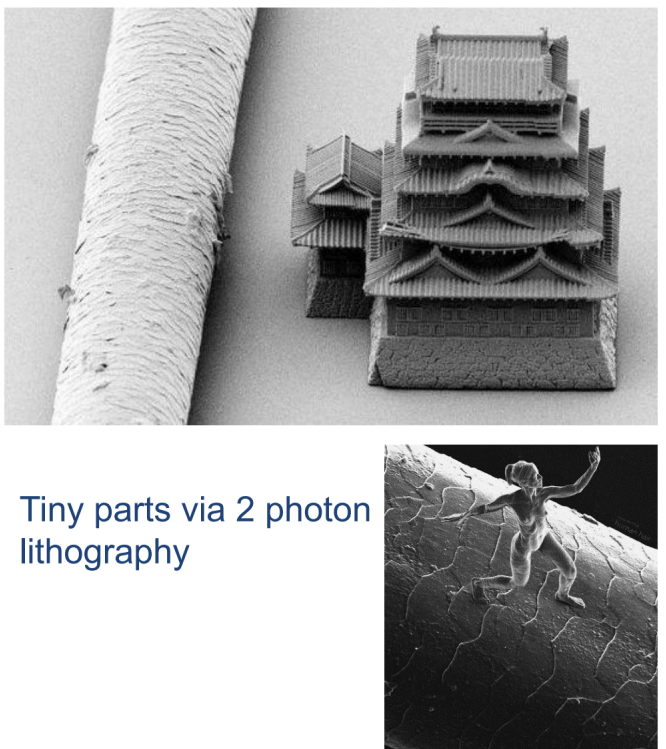
\includegraphics[width=0.4\textwidth]{assets/2photonpolymerization.png}
   \caption{2-Photon Polymerization (2PP)}
   \label{fig:2photonpolymerization.png}
  \end{figure}
\end{itemize}
Typisch worden UV-uithardende polymeren gebruikt maar sinds kort kan je ook metaal of keramiekdeeltjes in de hars brengen. Deze techniek biedt extreem hoge precisie en je kan er heel grote stukken mee maken, nadelen zijn wel dat na het printen je nog verder moet uitharden in een UV-oven, er zijn ook supports nodig en dat het materiaal instabiel blijft over tijd (door die zon, zage we eerder). Toepassingen zijn op maat gemaakte hoorapparaten, chirurgische mallen, zelfs 3D-geprinte zolen voor adidas schoenen, \dots
\begin{figure}[H]
  \centering
  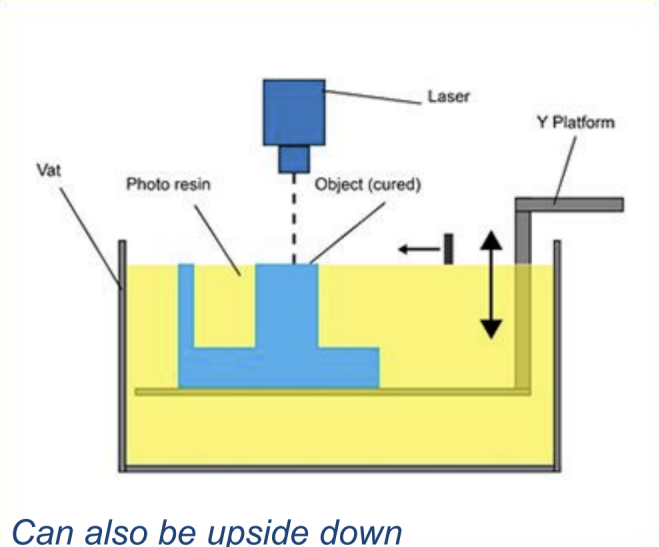
\includegraphics[width=0.5\textwidth]{assets/vatpolymerizatie.png}
  \caption{Vat polymerization}
  \label{fig:vatpolymerizatie.png}
 \end{figure}
\subsubsection{Powder bed fusion (poederbedsmelten)}
Hier wordt materiaal aangevoerd in de vorm van een poederbed, een roller spreidt een dunne laag poeder over het platform waarna een krachtige hittebron (laser- of elektronenstraal) de poederdeeltjes lokaal smelt/sintert. Het platform zakt dan zodat een nieuwe laag poeder wordt verspreid en het proces herhaalt. Bekende technieken zijn:
\begin{itemize}
  \item \textbf{Selective Laser Sintering (SLS):} Hierbij wordt een laser gebruikt om het poeder te smelten of sinteren. Meestal gebruikt voor polymeren zoals Nylon
  \item \textbf{Electron Beam Melting (EBM):} Hierbij wordt een elektronenstraal gebruikt, dit vereist een vacuümomgeving (dit maakt het sneller voor bepaalde metalen) en is vooral geschikt voor metalen met hoge smeltpunten.
  \begin{figure}[H]
    \centering
    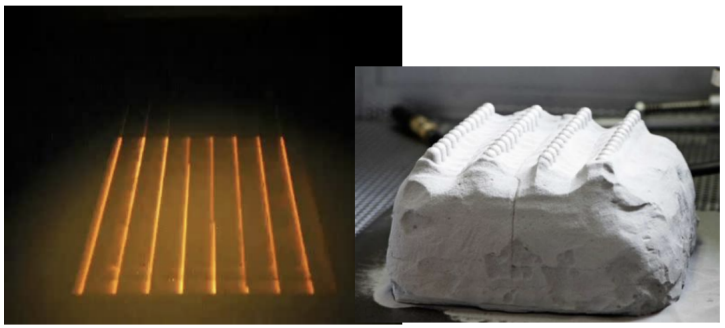
\includegraphics[width=0.6\textwidth]{assets/EBM.png}
    \caption{Electron Beam Melting (EBM)}
    \label{fig:EBM.png}
   \end{figure}
  \item \textbf{Laser Powder Bed Fusion (LPBF):} Dit is een meer algemene term die zowel SLS als Direct Metal Laser Sintering (DMLS) omvat, waarbij een laser wordt gebruikt om metalen poeders te smelten.
  \begin{figure}[H]
    \centering
    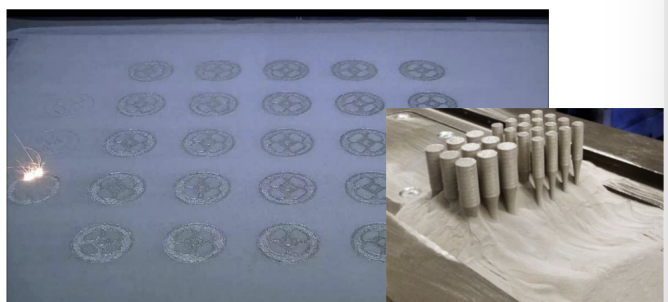
\includegraphics[width=0.6\textwidth]{assets/LPBF.png}
    \caption{Laser Powder Bed Fusion (LPBF)}
    \label{fig:LPBF.png}
   \end{figure}
  LBPF is nauwkeuriger, kan meerdere materialen gebruiken en heeft een snellere productietijd dan EBM maar LBPF heeft thermische restspanningen en is trager in het algemeen (spiegeltjes moeten draaien).
\end{itemize}
Er kan hier een breed scala aan materialen worden gebruikt; functionele metalen(stalen, titanium-, aluminium- en nikkellegeringen) en polymeren. Deze techniek maakt zeer sterke, direct functionele eindproducten met hoge complexiteit, maar een groot nadeel is een enorme opbouw van thermische restspanningen, dit is omdat elke laag kort en lokaal verhit wordt, dit is waarom deze sterk wilt krimpen tijdens het afkoelen, dit wordt tegengehouden door de vastzittende, reeds gekoelde onderlaag, wat kan leiden tot warping. Dit willen we ZEKER beperken, dit kan gedaan worden door het poederbed voor te verwarmen tot net onder de smelttemperatuur, er is ook ruwe oppervlakteafwerking door die poederdeeltjes die niet gesmelt zijn en aan de randen blijven kleven. Ontwerpvrijheid is vrijwel onbeperkt. Tegenwoordig kan je ook meerdere materialen tegelijk gebruiken.
\begin{figure}[H]
  \centering
  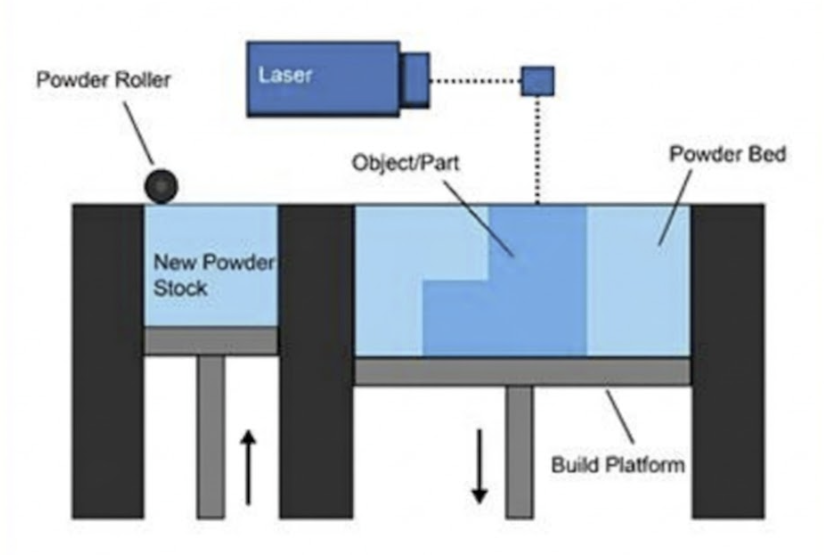
\includegraphics[width=0.5\textwidth]{assets/powerbedfusion.png}
  \caption{Powder bed fusion (poederbedsmelten)}
  \label{fig:powerbedfusion.png}
 \end{figure}
\subsubsection{Direct energy deposition (DED)}
Dit is niet met een poederbed, hier wordt het materiaal (in de vorm van metaalpoeder of metaaldraad) direct in een smeltbad gespoten of gevoerd. Dit smeltbad wordt gecreëerd door een krachtige hittebron zoals een laser of plasmastraal. Dit smeltbad en materiaaltoevoer bevinden zich op een robotarm, dit geeft het veel bewegingsvrijheid, want de printkop is nu in staat om de hele 3D-ruimte te gebruiken, niet meer beperkt tot 'laag-per-laag'. Bekende technieken zijn Laser Cladding en Wire Arc AM, voornamelijk wordt met metalen zoals staalsoorten, nikkellegeringen en titaniumlegeringen, maar het is ook geschikt om meerdere materialen te mixen (metal multimaterial of gradiënt materialen). Voordelen ziijn dat de productiviteit hoog ligt en enorm grote stukken gemaakt kunnen worden, de techniek is ook zeer geschikt voor onderdeelreparatie en is makkelijk combineerbaar met conventionele (substractieve) technieken waarbij je bvb eerst ruw print en dan glad freest, nadelen zijn wel dat er door hitte veel lokale thermische restspanningen onstaan wat kan leiden tot kromtrekken, en dat dus de oppervlaktekwaliteit slecht is, het kan ook geen kleine of fijne prints maken, het is ook niet mogelijk om supports te maken. Wordt gebruikt in de aerospace om bvb. raketten te maken.
\begin{figure}[H]
  \centering
  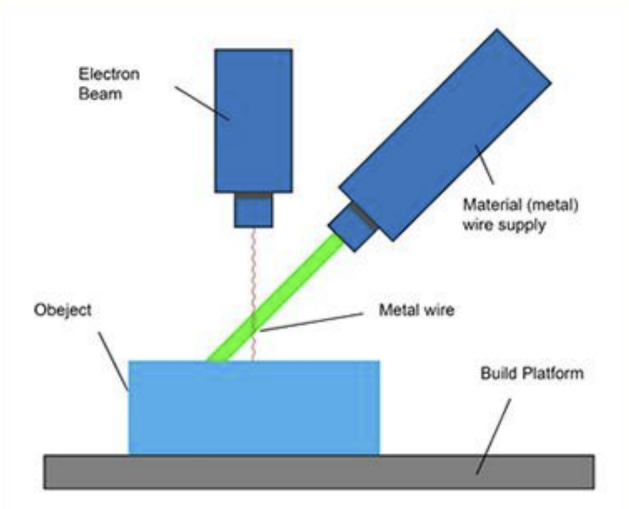
\includegraphics[width=0.5\textwidth]{assets/DED.png}
  \caption{Directed energy deposition (DED)}
  \label{fig:DED.png}
 \end{figure}